\section{Introduction}
A client dominated by one class must use a shared model that also serves nineteen other label distributions. In our label-skewed CIFAR-10 setting, the shared model reaches 38.96\% client-macro accuracy, below the 63.06\% obtained by predicting from local class frequencies alone. Figure~\ref{fig:motivation} motivates interpreting shared logits locally~\cite{mcmahan2017fedavg,arivazhagan2019fedper,chen2022fedrod}.

Fixed unit-strength prior addition uses a preset offset; vector scaling supplies no client-prior center~\cite{menon2021logitadjust,guo2017calibration}. Fixed addition can duplicate information in shared logits; an unconstrained fit must infer it from limited local labels.

We shrink the bias toward the client's prior instead of adding it. Infinite regularization fixes the prior offset; vanishing regularization removes the penalty. At an optimum, bias deviations track observed counts minus fitted probability mass: agreeing centers are retained and disagreeing ones corrected.

PR-LFL (prior-regularized lightweight federated learning) lowers NLL in each seed on both tasks. Class permutation isolates alignment; same-prior bias-corrected temperature scaling (BCTS) supports the center across score families. Local state costs 80 B; shared uploads cost 54,067 B.

\begin{figure}[!htb]\centering
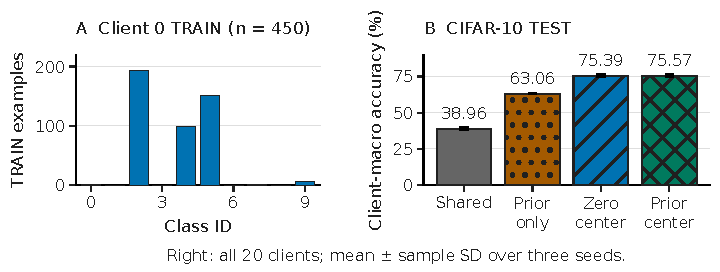
\includegraphics[width=\linewidth]{figures/motivation_route_a.pdf}
\caption{Local counts expose the prediction gap. Left: CIFAR client 0 TRAIN. Right: client-macro accuracy over twenty clients and three seeds, including prior-only prediction.}\label{fig:motivation}
\end{figure}

\paragraph{Contributions.}
\emph{A formulation that contains both baseline objectives as limits.} We treat the client's class prior as the center of a penalized post-hoc fit. $\lambda\to\infty$ recovers fixed logit adjustment, $\lambda\to0$ removes the penalty from the vector-scaling objective, and the optimum satisfies $\lambda(b-\mu)=n-\sum p$. The two standard objectives become penalty endpoints of one formulation instead of competitors.

\emph{An attribution control that needs no retraining.} Permuting the prior's class labels keeps its norm, the predictor's capacity, and the solver fixed, yet increases NLL relative to the aligned center in all 60 client-seed pairs per task, and the permuted predictor's mean NLL exceeds the zero-center mean on both tasks. The benefit comes from class alignment, not from shrinkage strength or extra parameters.

\emph{A deployment point at 54,067 B.} The same predictor fitted on logits from three-bit shared training stays within 0.03 accuracy points of the reported dense-training means on both tasks, with 90.1\% less uplink and 80 B of added local state.

\section{Related Work}
\paragraph{Personalization.}
FedProx, SCAFFOLD and FedNova change shared optimization~\cite{li2020fedprox,karimireddy2020scaffold,wang2020fednova}. FedPer/FedRoD retain personal heads; Ditto/pFedMe regularize personal models; FedBN retains local normalization~\cite{li2021ditto,dinh2020pfedme,li2021fedbn}. Quantization, sparsification and error feedback cut traffic~\cite{alistarh2017qsgd,stich2018sparsified,karimireddy2019errorfeedback}. PR-LFL fits frozen logits locally.

\paragraph{Class priors and label shift.}
EM and black-box shift estimation infer target priors~\cite{saerens2002prior,lipton2018bbse}. Logit adjustment, Balanced Softmax and FedLC use class counts in prediction or training~\cite{menon2021logitadjust,ren2020balanced,zhang2022fedlc}. PRIOR learns centers for Bregman-regularized model training~\cite{shi2023prior}; we center a convex frozen-logit predictor on observed log class frequencies.

\paragraph{Post-hoc calibration.}
Temperature/vector scaling, BCTS and Dirichlet calibration transform scores~\cite{guo2017calibration,alexandari2020labelshift,kull2019dirichlet}. LaSCal fits temperature using labeled source and unlabeled target data~\cite{popordanoska2024lascal}; our center uses client TRAIN labels. Calibration studies inform evaluation~\cite{vaicenavicius2019calibration,kumar2019verified,ovadia2019shift}. FedCal aggregates parameterized scalers~\cite{peng2024fedcal}; private multiclass calibration learns global scalers~\cite{maddock2025privatecal}. FedNPC retrains a server classifier on isotropic synthetic features and uniform labels~\cite{gao2026fednpc}; we fit client TRAIN logits with a prior-centered penalty. Prediction states stay local.
